% Latex template: mahmoud.s.fahmy@students.kasralainy.edu.eg
% For more details: https://www.sharelatex.com/learn/Beamer

\documentclass{beamer}					% Document class

\usepackage{tikz}
	\usetikzlibrary{math}
\usepackage[english]{babel}				% Set language
\usepackage[utf8]{inputenc}
\usepackage[T1]{fontenc}

\mode<presentation>						% Set options
{
  \usetheme{default}					% Set theme
  \usecolortheme{default} 				% Set colors
  \usefonttheme{default}  				% Set font theme
  \setbeamertemplate{caption}[numbered]	% Set caption to be numbered
  \beamertemplatenavigationsymbolsempty
}

\usepackage{graphicx}					% For including figures
\usepackage{booktabs}					% For table rules
\usepackage{hyperref}					% For cross-referencing
\usepackage{amsfonts}
\usepackage{amsthm}
\usepackage{newtxtext, newtxmath}
\usepackage[natbib, style=apa]{biblatex}
\addbibresource{references.bib}



%\newtheorem{theorem}{Theorem}
\newtheorem{proposition}{Proposition}
%\newtheorem{definition}{Definition}
%\newtheorem{lemma}{Lemma}
%\newtheorem{corollary}{Corollary}
%\newtheorem{example}{Example}
\newtheorem*{remark}{Remark}
\newtheorem*{assumption}{Assumption}

\def\f{\mathbb{F}}
\def\fp{\mathbb{F}_{p}}
\def\fq{\mathbb{F}_{q}}
\def\R{\mathbb{R}}
\def\N{\mathbb{N}}
\def\z{\mathbb{Z}}
\def\zp{\mathbb{Z}_p}
\def\zpx{\mathbb{Z}_p^*}
\def\fpx{\mathbb{F}_p^*}
\def\rem{ \% }
%\def\rem{\mbox{ rem }}
\def\a{\underline{a}}
\def\b{\underline{b}}
\def\c{\underline{c}}

\def\VAR{ \mbox {VAR} }
\newcommand{\Mod}[1]{\ (\mathrm{mod}\ #1)}

\newcommand{\subseq}[3]{#1[_{#2}^{#3}}
\newcommand{\cardinality}[1]{\#{#1}}



\newcommand{\Z}{\mathbb{Z}}


% \title{Comparing balanced \texorpdfstring{$\mathbb{Z}_v$}{Zv}-sequences obtained from \\
% ElGamal function to random balanced sequences}
\title{Randomness properties of $\mathbb{Z}_v$ ElGamal sequences}
\author{
Daniel Panario\texorpdfstring{$^*$}{*} \and 
Lucas Pandolfo Perin\texorpdfstring{$^\dagger$}{\dag} \and 
Brett Stevens\texorpdfstring{$^*$}{*}}
\institute{\texorpdfstring{$^*$}{*}Carleton University --- Canada \\ 
\texorpdfstring{$^\dagger$}{\dag}Universidade Federal de Santa Catarina --- Brazil \\
\texorpdfstring{$^\dagger$}{\dag}Technical Innovation Institute --- United Arab Emirates}
\date{2020-08-05}

% Uncomment this to have the outline at the beginning of each section highlighted.
\AtBeginSection[]
{
 \begin{frame}{Outline}
   \tableofcontents[currentsection]
 \end{frame}
}

\begin{document}

\begin{frame}
  \titlepage
\end{frame}

\begin{frame}{Outline}
  \tableofcontents
\end{frame}

\section{Contextualization}
    
\begin{frame}{Introduction}
    \begin{center}
        \emph{Sidon sets and statistics of the ElGamal function} \\
        \citet*{boppre2020sidon}
    \end{center}
    
    \begin{itemize}
        \item Started in 2016 as a research challenge by Joachim von zur Gathen;
        \item Boppré and Perin wrote a report with experimental analysis;
        \item By 2017, Ana and Joachim wrote the Sidon sets part and submitted to arxiv.
        \item In 2020, the paper was published in Cryptologia.
    \end{itemize}
\end{frame}


\begin{frame}{ElGamal Permutations}

\begin{center}
    Let 
    $$G = \Z_p^* = \{1, \ldots, p-1\}$$
    be a cyclic group of order $d =p-1$ $p$ prime and
    $$\Z_d = \{0, \ldots, d-1\}$$
\end{center}

    \pause
    \begin{itemize}
        \item ElGamal signatures use $G = \{ g^x : x\in \Z_d\}$, where $g$ is a generator of $G$;
        \item $g^x$ is a unique representation of $x$, and thus it spans a permutation of $G$.
        \item We want to investigate the randomness of the map $x \to g^x$
    \end{itemize}
    
\end{frame}


\begin{frame}{ElGamal Permutations}

\begin{center}
Since want to investigate permutations of $G$, we introduce the following notation.
\end{center}
\vspace{10pt}

\begin{minipage}{.5\textwidth}
	\begin{table}[]
	    \centering
	    \begin{tabular}{c|c}
	        $x$ & $x^\star$ \\ \hline \hline
	        $1$ & $1$ \\
	        $2$ & $2$ \\
	        $\cdots$ & $\cdots$ \\
	        $p-2$ & $p-2$ \\
	        $p-1$ & $0$ 
	    \end{tabular}
	     \caption{$\star: \mathbb{Z}_p^* \rightarrow \mathbb{Z}_d$}
	    \label{tab:xmap}
	\end{table}
\end{minipage}%
\begin{minipage}{0.5\textwidth}
    Now for $x\in G$, we can evaluate the map from $G$ to $G$
    $$x \to g^{x^\star}$$ 
     with respect to its cyclic properties.
\end{minipage}

    
\end{frame}



\begin{frame}{ElGamal Permutations}
Example: Let $p =5$, then $2$ and $3$ are generators of G = $\Z_p^*$.

    \begin{columns}
        \begin{column}{0.45\textwidth}
        \centering
            \begin{table}[]
    	    \begin{tabular}{c|c}
    	        $x$ & $g^{x^\star} $ \\ \hline \hline
    	        $1$ & $2^{1^\star} = 2$ \\
    	        $2$ & $2^{2^\star} = 4$ \\
    	        $3$ & $2^{3^\star} = 3$ \\
    	        $4$ & $2^{4^\star} = 1$  
    	    \end{tabular}
    	    \caption{cycles = \{\{1,2,4\},\{3\}\}}
    	    \label{tab:xmap1}
    	    \end{table}
        \end{column}
        \begin{column}{0.45\textwidth}
    	    \centering
            \begin{table}[]
    	    \begin{tabular}{c|c}
    	        $x$ & $g^{x^\star} $ \\ \hline \hline
    	        $1$ & $3^{1^\star} = 3$ \\
    	        $2$ & $3^{2^\star} = 4$ \\
    	        $3$ & $3^{3^\star} = 2$ \\
    	        $4$ & $3^{4^\star} = 1$
    	    \end{tabular}
    	    \caption{cycles = \{1,2,3,4\}}
    	    \label{tab:xmap2}
    	    \end{table}
        \end{column}
  \end{columns}
  
  \pause
  \begin{itemize}
      \item Distinct $g$ produce distinct permutations;
      \item Distinct $g$ affect the cyclic structures.
  \end{itemize}
  
  We will consider the $*$ implicit from now on and simply use $g^x$.
  
\end{frame}


\begin{frame}{Pictorial Representation}
    One fig here
\end{frame}

\begin{frame}{Pictorial Representation}
    Multiple figures here
\end{frame}

\begin{frame}{Number of cycles}
    \begin{figure}
        \centering
        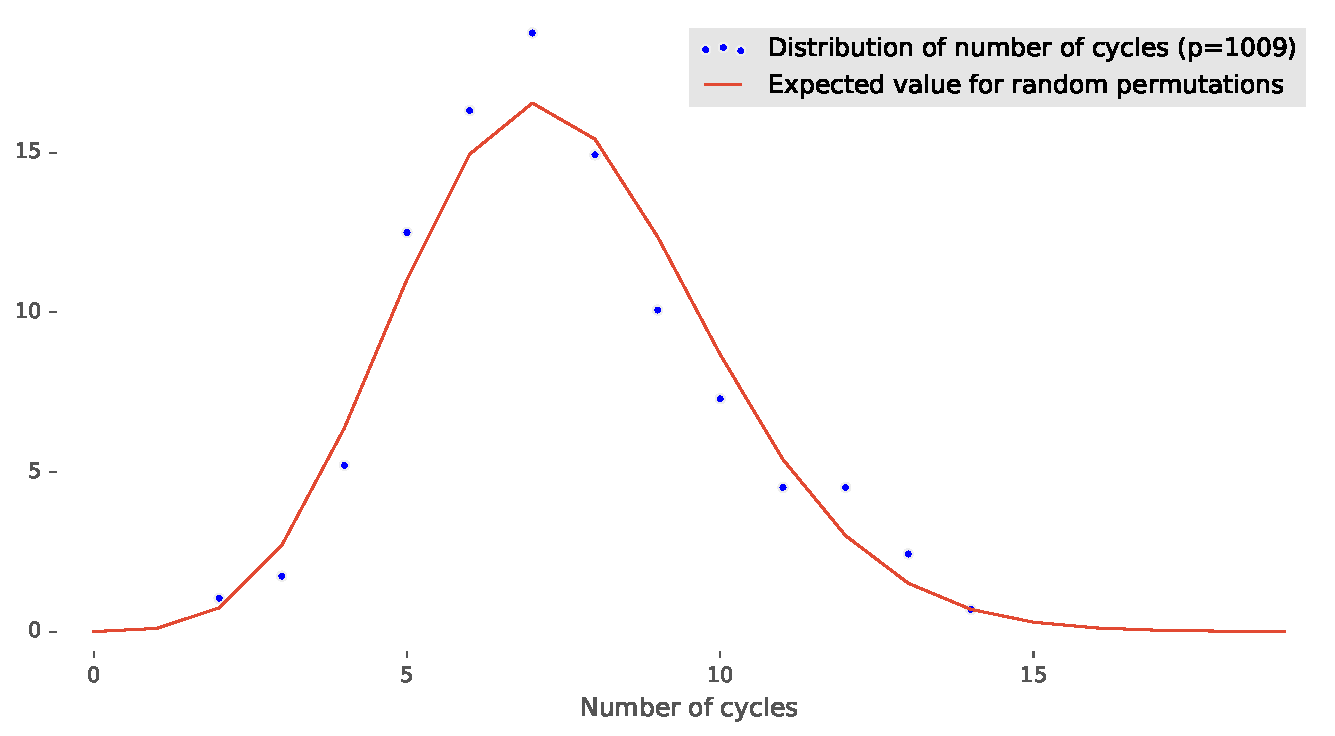
\includegraphics[width=\textwidth]{figures/distribution_of_number_of_cycles_p_1009}
        \caption{Distribution of number of cycles for all 288 generators of $\mathbb{F}_{1009}$}
        \label{fig:elgamalPermCycles}
    \end{figure}
\end{frame}

\begin{frame}{Number of $k$-cycles}
    \begin{figure}
        \centering
        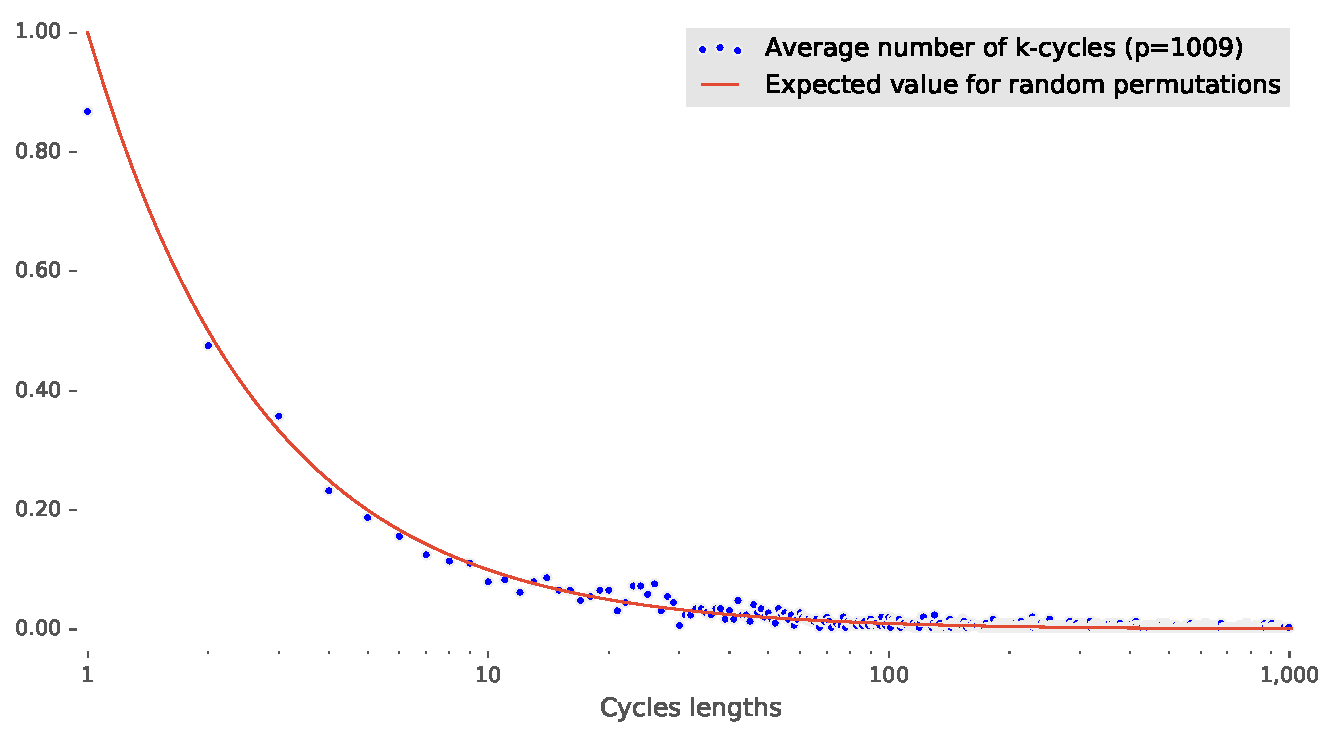
\includegraphics[width=\textwidth]{figures/average_number_of_k_cycles_p_1009}
        \caption{Average number of $k$-cycles in $\mathbb{F}_{1009}$}
        \label{fig:kcycles}
    \end{figure}
\end{frame}

\begin{frame}{Number of fixed points ($k=1$)}
    \begin{figure}
        \centering
        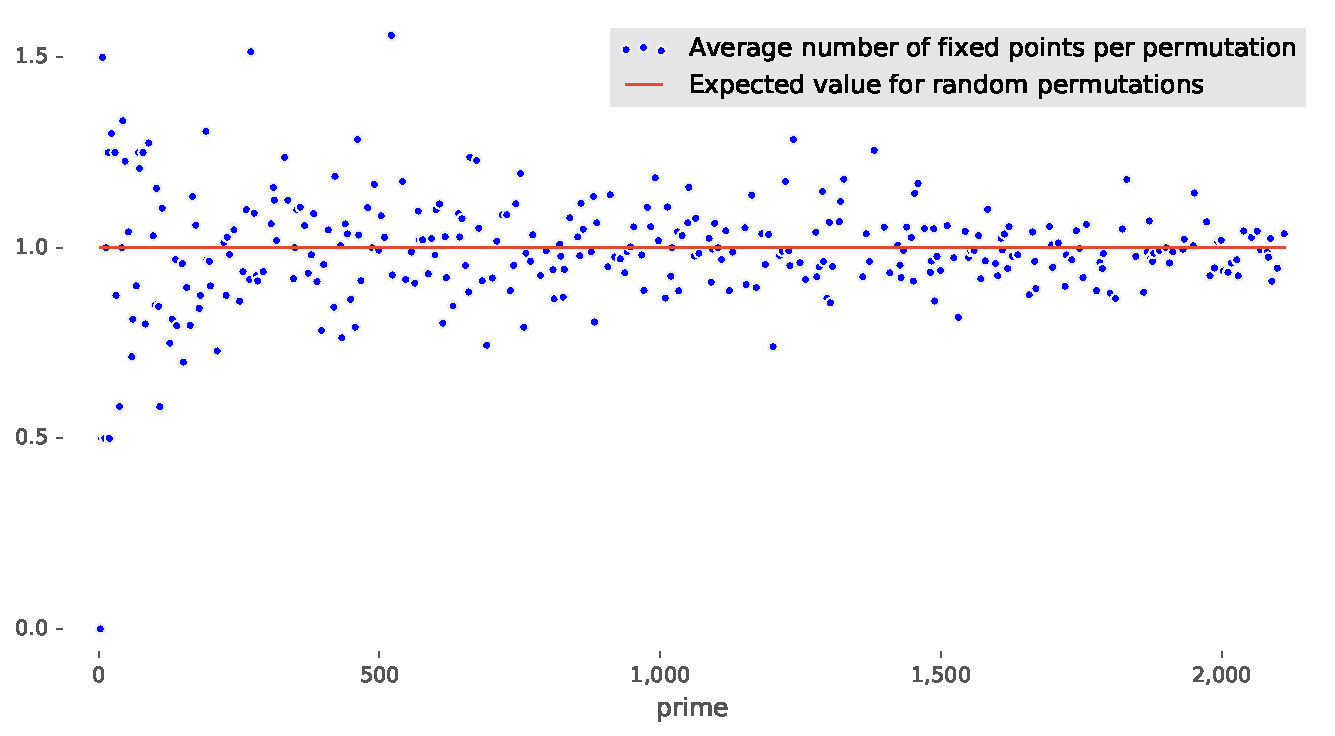
\includegraphics[width=\textwidth]{figures/average_number_of_fixed_points_per_permutation}
        \caption{Average number of fixed points in the generators of $\mathbb{F}_p$}
        \label{fig:fixedpoints}
    \end{figure}
\end{frame}


\begin{frame}{Results with Sidon Sets}
\end{frame}



\begin{frame}{Sequences from permutations}
    For some random permutation $\pi$ in $\mathbb{Z}_p^*$, a $v$-ary sequence $\pi_v\in\mathbb{Z}_v$ is obtained by reducing the permutation modulo $v$:
    \[
        \pi_v = (\pi_0 \rem v, \ldots, \pi_{p-2}\rem v).
    \]
    
    \pause
    \begin{align*}
        \pi &= ( 1, 3, 4, 2) \in \mathbb{Z}_5^*\\
        \pi_2 &= (1, 1, 0, 0) \in \mathbb{Z}_2
    \end{align*}
\end{frame}


\begin{frame}{ElGamal sequences from ElGamal permutations}
    We can do the same for ElGamal Permutations. For some ElGamal permutation $\gamma$ in $\mathbb{Z}_p^*$, a $v$-ary sequence $\gamma_v\in\mathbb{Z}_v$ is obtained by reducing the ElGamal permutation modulo $v$:
        \[
            \gamma_v = (\gamma_0 \rem v, \ldots, \gamma_{p-2}\rem v).
        \]
        
        \pause
        For $g = 2$ and $p = 5$, we have
        \begin{align*}
            \gamma &= ( (2^0) \rem 5) \rem 2, \ldots, (2^3) \rem 5) \rem 2) = (1, 2, 4, 3) \in \mathbb{Z}_5^*\\
            \gamma_2 &= (1, 0, 0, 1) \in \mathbb{Z}_2
        \end{align*}
\end{frame}

\begin{frame}{Randomness properties of ElGamal Sequences?}
    
    \begin{center}
        How closely do ElGamal sequences compare to random balanced sequences over $\mathbb{Z}_v$?
    \end{center}
    
    \begin{itemize}
        \item Balance
        \item Period length
        \item Distribution of \emph{tuples} of length $t$  
        $$\lambda(z) = \cardinality{\{i \in [0,p-1]: \sigma(i+_{n} \iota) = z(\iota),\; 0 \leq \iota < t\}}$$
        \item  Distribution of \emph{runs} of length $t$
        \begin{align*}
            \rho(b,t) = & \cardinality{ \{i \in [0,p-1]: }\\
                        &\sigma(i-_{n} 1),\sigma(i+_n t) \neq b = \sigma(i+_n\iota),\; 0 \leq \iota < t\}
        \end{align*}
        % $\rho(b,t) = \cardinality{ \{i \in [0,p-1]: \sigma(i-_{n} 1),\sigma(i+_n t) \neq b = \sigma(i+_n\iota),\; 0 \leq \iota < t\}}$
    \end{itemize}
  
  \end{frame}

% \begin{frame}{ElGamal Sequences}

% An {\em ElGamal sequence} is obtained by reducing an ElGamal permutation modulo $v$:
  
%   \[\gamma_v = ((g^0\rem p)\rem v,(g^1\rem p)\rem v,(g^2\rem p)\rem v,(g^3\rem p)\rem v,\ldots)\]

  

% \end{frame}




% \begin{frame}{Randomness properties of ElGamal Sequences?}
%   \begin{itemize}
%   \item Balance
%   \item Period
%   \item   $\lambda(z) = \cardinality{\{i \in [0,p-1]: \sigma(i+_{n} \iota) = z(\iota),\; 0 \leq \iota < t\}}$
%     \item  $\rho(b,t) = \cardinality{ \{i \in [0,p-1]: \sigma(i-_{n} 1),\sigma(i+_n t) \neq b = \sigma(i+_n\iota),\; 0 \leq \iota < t\}}$
%     \end{itemize}
  
%   \end{frame}


\begin{frame}{ElGamal Run ratio Experiment}
    Show experiment with ratio against expected from Golomb's postulates
\end{frame}



 	

%%% Local Variables:
%%% TeX-master: "../main.tex"
%%% End:


\section{Bounds for random \texorpdfstring{$v$}{v}-ary sequences}
    
    \begin{frame}{Balance}

      The number of $x \equiv i \mod v$ in $[1,p-1]$ is
      \[ \lceil (p-1 - ((i-1) \bmod v))/v\rceil\]

\begin{proposition} \label{balancedproperty}
Let $\pi$ be a permutation in $\zpx$, then $\pi_v$ is a balanced 
sequence over $\z_v$ if and only if $v \mid p-1$.
\end{proposition}
      
      \end{frame}


      \begin{frame}{Period}

        \begin{lemma} \label{lemma_near_balanced_period}
If $p \equiv \alpha \neq 1 \Mod v$, then $\pi_v$ has period $N =p-1$ for any $\pi: \zpx \rightarrow \zpx$.
\end{lemma}
\begin{proof}

  The difference in the number of occurences of any two symbols must be a multiple of $(p-1)/N$. But   
  \[
    |\pi_v|_a = \begin{cases} \lceil (p-1)/v \rceil &  0 \leq a < \alpha -1, \\
      \lfloor (p-1)/v \rfloor & \mbox{otherwise}.
    \end{cases}
  \]
\end{proof}

\end{frame}

\begin{frame}{Period}


\begin{theorem}For every $\epsilon >0 $ there exists an $n_{\epsilon}$ so that for 
  all $p \geq n_{\epsilon}$, the number $T$ of permutations $\pi_v$ with period 
  $p-1$ satisfies 
  \begin{equation} \label{T_bound_epsilon}
    (p-1)!(1-\epsilon) \leq T \leq (p-1)!.
  \end{equation}
\end{theorem}
  
\end{frame}


\begin{frame}{Special case}

  When $q$ is prime and $p=vq+1$,
  \[
    (p-1)! - T = v!(q!)^v 
    \]

    This includes the case of Sophie Germain primes.
  
  \end{frame}

  \begin{frame}{de Bruijn graph}
    \usetikzlibrary {arrows.meta}
    \begin{center}
      \begin{tikzpicture}
%        [->,>={Stealth[round]},shorten >=1pt,auto,node distance=2.8cm,on grid,semithick]
        [->,>={Stealth[round]},auto,node distance=2.8cm,very thick]
      \node (00) at  (0,0) [circle,draw=black,line width=1.0mm] {00};
      \node (01) at  (-2,2) [circle,draw=black,line width=1.0mm] {01};
      \node (10) at  (2,2) [circle,draw=black,line width=1.0mm] {10};
      \node (11) at  (0,4) [circle,draw=black,line width=1.0mm] {11};

      \path (00) edge [loop below] (00);
      \path (00) edge (01);
      \path (10) edge (00);
      \draw (10) to[out=150,in=30]  (01);
      \draw (01) to[out=-30,in=-150]  (10);
      \path (01) edge (11);
      \path (11) edge (10);
      \path (11) edge [loop above] (11);
    \end{tikzpicture}
    \end{center}

  \end{frame}

  \begin{frame}{Transfer Matrix}


    
    Transfer matrix is directed adjacency matrix of de Bruijn graph with variables
    \[
      T =  \bordermatrix{ & 00 & 01 & 10 & 11 \cr
     00 & ux_0 & ux_0 & 0 & 0 \cr
     01 & 0 & 0 & x_0 & x_0 \cr
     10 & 1 & 1 & 0 & 0\cr
   11 & 0 & 0 & 1 & 1}
      \]

\[
      C =  \bordermatrix{ & 00 & 01 & 10 & 11 \cr
     00 & 1 & 0 & 0 & 0 \cr
     01 & 0 & 1 & 0 & 0 \cr
     10 & 0 & 0 & 1 & 0\cr
   11 & 0 & 0 & 0 & 1}
      \]

\[
  \sum_{\mathbf{k} \in \mathbb{N}^t} a_n(k)x^{\mathbf k} = \sum_{z',z'' \in \z_v^t} C_{z',z''} T^{n}_{z',z''}.
\]
      
\end{frame}


 	

%%% Local Variables:
%%% TeX-master: "../main.tex"
%%% End:



\section{Bounds for ElGamal \texorpdfstring{$v$}{v}-ary sequences}
    
\begin{frame}{Balance}

\begin{proposition} \label{balancedproperty}
Let $\pi$ be a permutation in $\zpx$, then $\pi_v$ is a balanced 
sequence over $\z_v$ if and only if $v \mid p-1$.
\end{proposition}

  
\end{frame}

\begin{frame}{Period}

\begin{theorem}
The ElGamal sequence $\gamma_v$ has period $N = p-1$.
\end{theorem}

\begin{proof}
  \begin{enumerate}
  \item $p \not\equiv 1 \Mod v$:  Use balance
  \item $p \equiv 1 \Mod v$: Suppose period $N < p-1$: $g^{i+N}\rem p \equiv_v g^i \rem p$ 
  \item Let $i=0$:  $g' = g^N\rem p  \equiv_v 1$.
  \item Let $p = kg'+r$, $x = k+1$ ($p < xg' < 2p$). Let $i = \log_g(x)$:
    \[x \equiv_v xg'\rem p = xg'-p \equiv_v xg' -1\]
  \item $x (g'-1) \equiv_v 1 \equiv_v g'$ is a contradiction.
\end{enumerate}
\end{proof}

  
\end{frame}

\begin{frame}{Tuples}

  
\begin{theorem}\label{elgamal_tuple}
  Let $\gamma_v$ be an ElGamal sequence and $p = q g^{t-1} + r$, then
  \[
     \left \lfloor \frac{g}{v} \right \rfloor^{t-1} 
     \left \lfloor\frac{q}{v} \right \rfloor 
\leq \lambda(z) 
\leq \left \lceil \frac{g}{v} \right \rceil^{t-1} 
     \left(\left \lfloor\frac{q}{v} \right\rfloor +1 \right).
  \]
\end{theorem}



  
\end{frame}

\begin{frame}{Proof}
  \[
    X = \left \{x \in [1,p-1]: (g^i x) \rem p \equiv_v z_i, 0 \leq i < t \right \}
    \]

Let $c_i = g^{i}z_{0} - z_{i}$, $0 \leq i < t$.
  \[
    D = \{d \in \z^t:d_0 = 0,  d_i \equiv_v \alpha^{-1}c_i\mbox{ and } 
          gd_{i-1} \leq d_i < g(d_{i-1}+1) \mbox{ for } 0 < i < t  \}.
  \]
  For $d \in D$, let\[
    X_{d} = \left \{x \in \z: x \equiv_v z_0,\; \frac{d_{i}p}{g^i} 
    \leq x < \frac{(d_{i}+1)p}{g^i}, \mbox{ for } 0 \leq i < t \right \}.
  \]
 
  \begin{align*}
\mbox{\Large Claim:         } \hspace{3cm} &   X = \bigcup_{d \in D} X_d & \hspace{4cm}
  \end{align*}


\end{frame}

\begin{frame}{$X_d \subset X$}

If $x \in X_{d}$, then $x \equiv_v z_0$ and 
  \[
    d_{i}p \leq g^ix < (d_{i}+1)p 
  \]
  Thus 
  \begin{align*}
    g^ix \rem  p &= g^ix-d_{i}p 
                \equiv_v g^ix-\alpha d_i 
                \equiv_v g^iz_0 - c_i 
                \equiv_v g^iz_0 - (g^iz_0 - z_i) = z_i,
  \end{align*}

  So $x \in X$.



\end{frame}

\begin{frame}{$X \subset \cup X_d$}

  For $x \in X$, define $g^ix = q_ip + r_i$:
\begin{align*}
&  q_0 = 0 \\
&  r_i = g^ix - q_ip = (g^ix) \rem p \equiv_v z_i \\
&  \frac{q_{i}p}{g^i} \leq x < \frac{(q_{i}+1)p}{g^i}
  \end{align*}

  So $x \in X_{(q_0,\ldots,q_{t-1})}$



\end{frame}

\begin{frame}{$X \subset \cup X_d$}


  \begin{align*}
    q_i &\equiv_v \alpha^{-1}q_ip  
          = \alpha^{-1}(g^ix - r_i )
          \equiv_v \alpha^{-1}(g^iz_0 - z_i) = \alpha^{-1}c_i.
  \end{align*}
Then,
  \begin{align*}
    q_i &= \frac{g^ix-r_i}{p} = \frac{g(g^{i-1}x)-r_i}{p}
          = \frac{g(q_{i-1}p+r_{i-1}) - r_i}{p} \\
        &= gq_{i-1} + g\frac{r_{i-1}}{p} -\frac{r_i}{p} 
          < g(q_{i-1}+1),
  \end{align*}
and
  \[
  gq_{i-1} = \frac{gq_{i-1}p}{p} \leq \frac{g(q_{i-1}p+r_{i-1})}{p} 
           = \frac{g(g^{i-1}x)}{p} = \frac{g^ix}{p} = q_i + \frac{r_i}{p}.
  \]
Since $gq_{i-1}, q_{i} \in \mathbb{Z}$ and $r_{i}/p < 1$, $\Rightarrow q_{i} \geq g q_{i-1}$.

Thus  $(q_0,\ldots,q_{t-1}) \in D$.


\end{frame}

\begin{frame}{Final step}

  \begin{align*} 
    X = \bigcup_{d \in D}X_d &= \bigcup_{d \in D} \left (\{x \equiv_v z_0 \} \bigcap 
        \left( \bigcap_{0 \leq i < t} \left \{\frac{d_ip}{g^i} 
                               \leq x < \frac{(d_i+1)p}{g^i} \right\} \right) \right). \\
    &=  \bigcup_{d \in D}
    \left (   \{x \equiv_v z_0 \} \cap \left \{\frac{d_{t-1}p}{g^{t-1}} 
    \leq x < \frac{(d_{t-1}+1)p}{g^{t-1}} \right \}\right). 
  \end{align*}

  \[
    \begin{array}{rcccl}
    \lfloor g/v \rfloor^{t-1}  &\leq &\cardinality{D} &\leq& \lceil g/v \rceil^{t-1} \\
    q &\leq &\cardinality{[d_{t-1}p/g^{t-1},(d_{t-1}+1)p/g^{t-1})} &\leq &q+1 \\
      \lfloor q/v \rfloor &\leq& \cardinality{X_d} &\leq& \lceil (q+1)/v \rceil
                            \end{array}
   \]

  \[
     \left \lfloor \frac{g}{v} \right \rfloor^{t-1} 
     \left \lfloor\frac{q}{v} \right \rfloor 
\leq \lambda(z) 
\leq \left \lceil \frac{g}{v} \right \rceil^{t-1} 
     \left(\left \lfloor\frac{q}{v} \right\rfloor +1 \right).
   \]
  
\qed
   
\end{frame}

\begin{frame}{Observations}

  \begin{itemize}
  \item When $g=mv$ bounds differ by at most $m^t$
    \item When $g=v$, $\left \lfloor\frac{q}{v} \right \rfloor \leq \lambda(z) \leq   
      \left \lfloor\frac{q}{v} \right\rfloor +1$
    \item If $p \geq v g^{t-1}$ and $g \geq v$, then $\lambda(z) > 0$ for all $z \in \z_v^t$
    \item If $\lambda(z) > 0$ for all $z \in \z_v^t$, then $g \geq v$ and $p \geq v^t+1$.
    \item Coincide when $g=v$
      \item $\gamma_v(i+1) \equiv_v g\gamma_v(i)- s$ for some $ 0 \leq s < g$.
    \end{itemize}
  
\end{frame}

\begin{frame}{Runs}
\begin{theorem}\label{elgamal_run}
Let $\gamma_v$ be an ElGamal sequence and $p = q g^{t-1} + r$.  For $z \in \z_v^t$, let 
  \[
    \mu(z) = \cardinality{\{ i \in [1,p-1]:\; g^{i+j}\rem p \equiv_v z_j,\; 0 \leq j < t-1,
                    \; g^{i+t-1}\rem p \not\equiv_v z_{t-1}\}}.
                \]
                Then
  \[
    \left \lfloor \frac{g}{v} \right \rfloor^{t-2} \left \lfloor \frac{(v-1)g}{v} \right \rfloor \left \lfloor\frac{q}{v} \right \rfloor \leq \mu(z) \leq  \left \lceil \frac{g}{v} \right \rceil^{t-2} \left \lceil \frac{(v-1)g}{v} \right \rceil\left(\left \lfloor\frac{q}{v} \right\rfloor +1 \right).
  \]
\end{theorem}
  
\end{frame}

\begin{frame}{Corollary}

  Let $p = q_t g^{t} + r_t$ and $p = q_{t+1} g^{t+1} + r_{t+1}$.  Then
\begin{multline*}
\left \lfloor \frac{g}{v} \right \rfloor^{t-1}\left \lfloor \frac{(v-1)g}{v} \right \rfloor \left \lfloor \frac{q_t}{v}\right \rfloor - \left \lceil \frac{g}{v} \right \rceil^{t}\left \lceil \frac{(v-1)g}{v} \right \rceil \left \lceil \frac{q_{t+1}+1}{v} \right \rceil  \\
\leq  \rho(b,t) \leq \\
\left \lceil \frac{g}{v} \right \rceil^{t-1}\left \lceil \frac{(v-1)g}{v} \right \rceil \left \lceil \frac{q_{t}+1}{v} \right \rceil - \left \lfloor \frac{g}{v} \right \rfloor^{t}\left \lfloor \frac{(v-1)g}{v} \right \rfloor \left  \lfloor \frac{q_{t+1}}{v} \right \rfloor,
\end{multline*}
and
  \[
    (v-1) \left \lfloor \frac{g}{v} \right \rfloor^{t} \left \lfloor \frac{(v-1)g}{v} \right \rfloor\left \lfloor\frac{q}{v} \right \rfloor \leq \rho(b,t) \leq  (v-1)\left \lceil \frac{g}{v} \right \rceil^{t}\left \lceil \frac{(v-1)g}{v} \right \rceil \left \lceil\frac{q+1}{v} \right\rceil.
  \]
  
\end{frame}

\begin{frame}{Comparison to random balanced sequences}

From theoretical results
  
  \begin{itemize}
    \item Balance matches exactly
  \item Periodicity matches very closely
  \item To first order, the number of tuples and runs matches
  \item To first order $\rho(t) \approx v \rho(t+1)$
  \end{itemize}
  
  
\end{frame}




%%% Local Variables:
%%% TeX-master: "../main.tex"
%%% End:

    
\section{Experimental results}
    
\begin{frame}{Experiment settings}

    We run experiments over two distinct data sets of pairs $(p, v)$ with $p > 1,000,000$ and $2 \leq v \leq 8$.
    
    \begin{description}
        \item[all primes:] Primes where $v \mid p -1$.
        \item[$g = v$ primes:] Primes where $v \mid p -1$ and $v$ is a generator.
    \end{description}

    \pause
    \begin{table}[ht]
    \centering
    \begin{tabular}{lrr}
        \toprule
                                  & all  &  $g = v$  \\ \midrule
        \# pairs $(p, v)$      & 715  & 400       \\ 
        \# distinct $v$           & 7    & 4         \\
        \# distinct primes        & 322  & 323       \\ 
        \# $v$ per prime (average) & 4.51 & 1.48      \\ \bottomrule
    \end{tabular}
    \label{tab:experiments}
\end{table}
    
    \begin{itemize}
        \item We run experiments over \emph{all primes} for the smallest 10 generators.
        \item If $v\in\{4,5,8\}$ then $v\neq g$.
    \end{itemize}
\end{frame}

\begin{frame}{ElGamal Sequences tuples lower and upper bounds}
    \begin{columns}
        \begin{column}{0.45\textwidth}
        \begin{center}
            All primes.
        \end{center}
            \begin{figure}
                \centering
                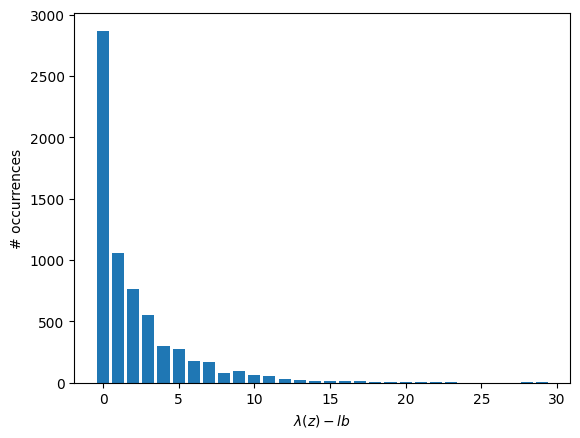
\includegraphics[width=\textwidth]{figures/LB0t2with012outliers.png}
            \end{figure}
        \end{column}
        \begin{column}{0.45\textwidth}
        \begin{center}
            $g = v$ primes.
        \end{center}
            \begin{figure}
                \centering
                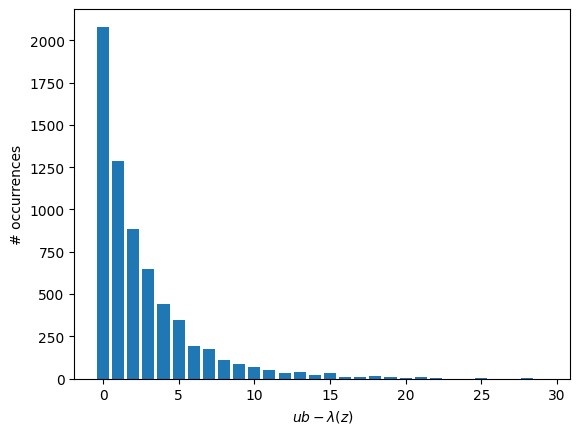
\includegraphics[width=\textwidth]{figures/UBt2with005outliers.png}
            \end{figure}
        \end{column}
    \end{columns}
    \begin{center}
                Distribution of $\rho(t+1)v/\rho(t)$ as a heatmap
    \end{center}
\end{frame}

\begin{frame}{ElGamal Sequences tuples lower and upper bounds}
    \begin{tabular}{ccc}
        a & Lower bounds & Upper bound \\
        $t = 2$ & 
        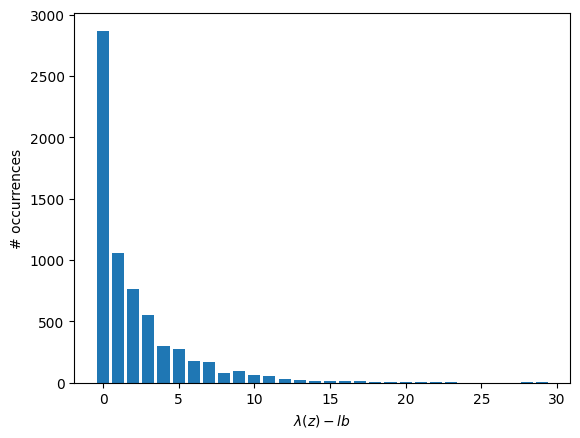
\includegraphics[width=0.3\textwidth]{figures/LB0t2with012outliers.png} &
        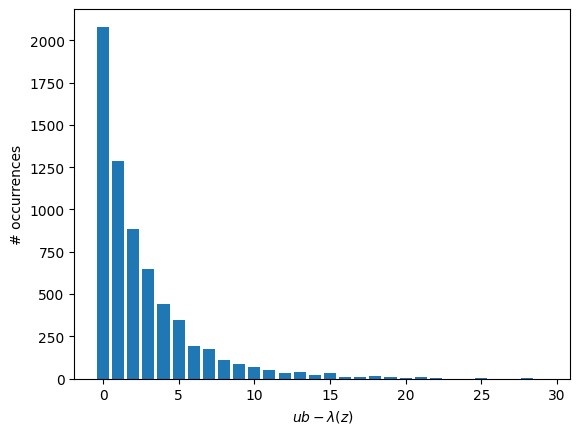
\includegraphics[width=0.3\textwidth]{figures/UBt2with005outliers.png} \\
        $t = 7$ & 
        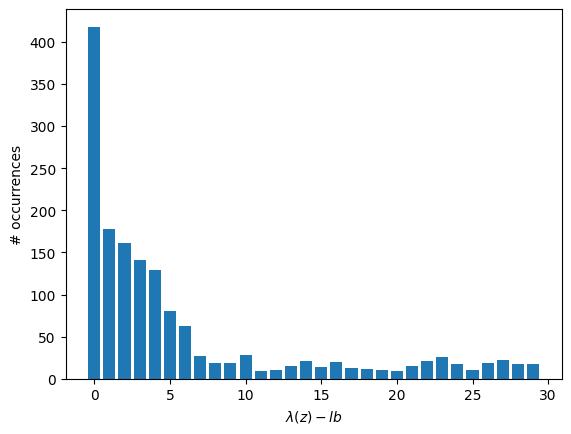
\includegraphics[width=0.3\textwidth]{figures/LB0t7with5975outliers.png} &
        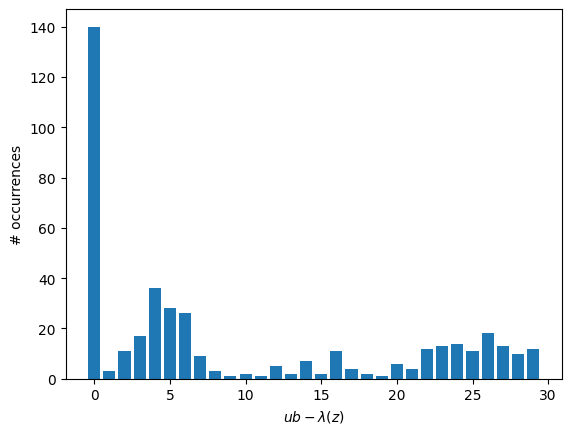
\includegraphics[width=0.3\textwidth]{figures/UBt7with9356outliers.png} 
    \end{tabular}
    \begin{center}
                Distribution of $\rho(t+1)v/\rho(t)$ as a heatmap
    \end{center}
\end{frame}


\begin{frame}{ElGamal Sequences run ratio Experiment}
    \begin{columns}
        \begin{column}{0.45\textwidth}
        \begin{center}
            All primes.
        \end{center}
            \begin{figure}
                \centering
                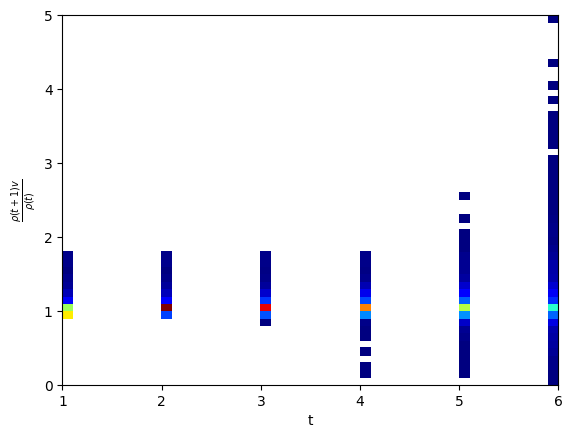
\includegraphics[width=\textwidth]{figures/AllDataNormalizedrunratio.png}
            \end{figure}
        \end{column}
        \begin{column}{0.45\textwidth}
        \begin{center}
            $g = v$ primes.
        \end{center}
            \begin{figure}
                \centering
                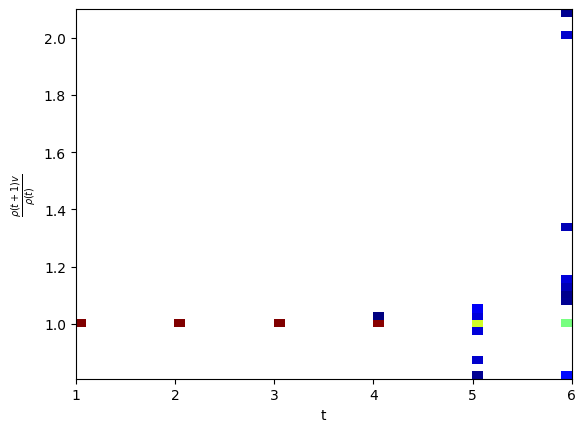
\includegraphics[width=\textwidth]{figures/AllDataAndvisGenNormalizedrunratio.png}
            \end{figure}
        \end{column}
    \end{columns}
    \begin{center}
                Distribution of $\rho(t+1)v/\rho(t)$ as a heatmap with $2 \leq v \leq 8$
    \end{center}
\end{frame}

\begin{frame}{ElGamal Sequences run ratio Experiment}
    \begin{columns}
        \begin{column}{0.45\textwidth}
        \begin{center}
            All primes.
        \end{center}
            \begin{figure}
                \centering
                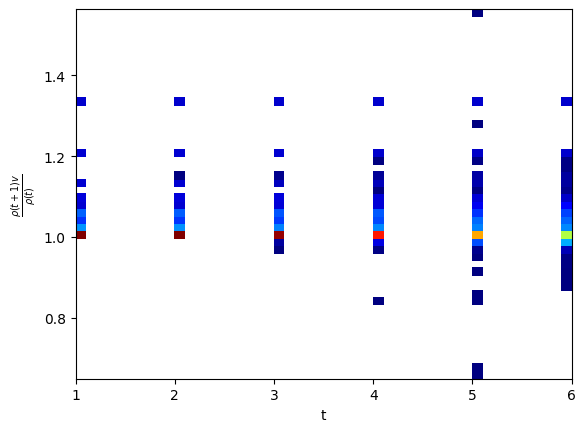
\includegraphics[width=\textwidth]{figures/v2Normalizedrunratio.png}
            \end{figure}
        \end{column}
        \begin{column}{0.45\textwidth}
        \begin{center}
            $g = v$ primes.
        \end{center}
            \begin{figure}
                \centering
                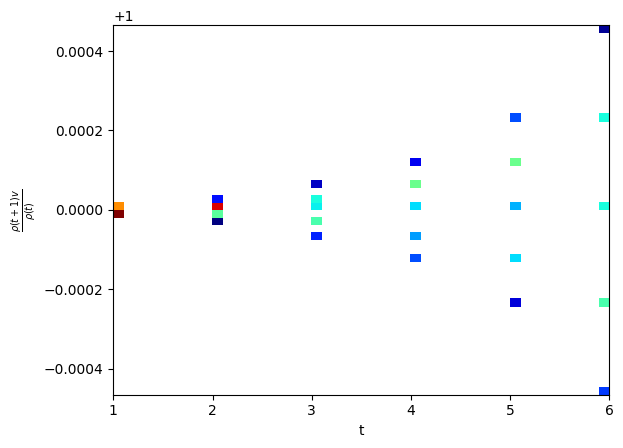
\includegraphics[width=\textwidth]{figures/v2AndvisGenNormalizedrunratio.png}
            \end{figure}
        \end{column}
    \end{columns}
    \begin{center}
                Distribution of $\rho(t+1)v/\rho(t)$ as a heatmap with $v = 2$
    \end{center}
\end{frame}


    
\section{Final Remarks}
    \begin{frame}{Conclusions}

  \begin{itemize}
    \item ElGamal permutations behave like random for cycle sizes and distribution of graph
    \item ElGamal permutations are close to random permutations for nonlineaity
    \item ElGamal sequences have balance and periodicity close to random
    \item Tuples in ElGamal sequences are distributed as in random balanced sequences
    \item Run lengths in ElGamal sequences satisfy Golomb's Randomness Postulate
    \end{itemize}
  
\end{frame}

\begin{frame}{Next steps}

  \begin{itemize}
  \item Experiments indicate that $\lambda(z)$ bounds are tight.  So any improvements will be conditional
  \item Prove properties of the distribution of $\lambda(z)$
  \item Prove linear complexity results for ElGamal sequences
  \item Determine expected linear complexity for random balanced random sequences
  \item Further investigate auto-correlation
    \item Will these be enough to justify cryptographic utility? 
    \end{itemize}
  
\end{frame}


\begin{frame}{}

  \begin{center}
  \scalebox{3}{Obrigado} \\

  \scalebox{3}{Thanks} \\

  
  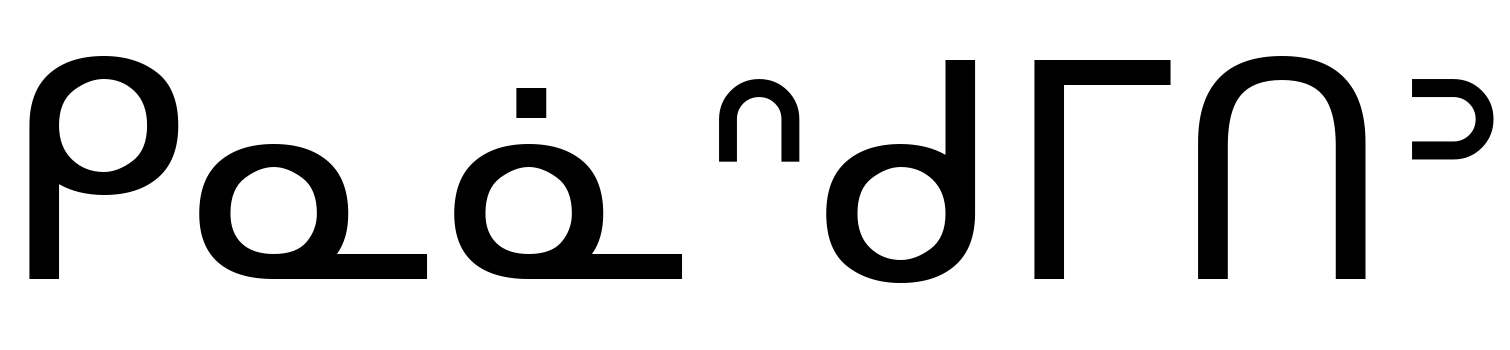
\includegraphics[width=5cm]{kinanaskomitin.png}

  
  
  
\includegraphics[width=6cm]{shukran_lak.png}
\end{center}
  
  
\end{frame}




%%% Local Variables:
%%% TeX-master: "../main.tex"
%%% End:

    
\section{References}


\begin{frame}[allowframebreaks]{References}
	\tiny
    % \bibliography{references}
	\printbibliography
\end{frame}

\end{document}


%%%Local Variables:
%%% mode: latex
%%% TeX-master: t
%%% eval: (TeX-PDF-mode 1)
%%% ispell-local-dictionary: "en_CA"
%%% eval: (flyspell-mode 1)
%%%End: